\documentclass[a4paper]{article}

\usepackage[toc,page]{appendix}

\usepackage[spanish]{babel}
\usepackage[utf8]{inputenc}
\usepackage{amsmath}
\usepackage{graphicx}
\usepackage{fancyhdr}
\usepackage{amsmath}
\usepackage[colorinlistoftodos]{todonotes}
\usepackage{xcolor}
\usepackage{minted}
\usepackage[font=small,labelfont=bf]{caption}
\usepackage{enumitem}
\setlist{nosep}

\usepackage{hyperref}

\hypersetup{
    colorlinks,
    citecolor=blue,
    filecolor=blue,
    linkcolor=blue,
    urlcolor=blue
}

\usepackage{geometry}
\geometry{a4paper}

\begin{document}
\begin{figure}
\centering

\includegraphics[scale=1]{./img/logo-facu}
\end{figure}

\title{\large\textsc{66.17 - Sistemas Digitales}\\
\large Trabajo Práctico 1 - Contador BCD de 4 dígitos con salida a display 7 segmentos}

\author{
Andrew Parlane \\
}

\maketitle

\newpage

\tableofcontents

\listoffigures

\newpage

\section{Introducción}

El objetivo de este trabajo es a diseñar, simular y implementar en FPGA un circuito digital que cuenta en código binario decimal (BCD para binary coded decimal) desde cero hasta 9999 y muestra el valor corriente en cuatro displays de siete segmentos.

Diseñé el circuito para funcionar con una Altera DE2 placa de desarrollo que tiene un cyclone II 2C35 FPGA. Para el propósito de este trabajo la única diferencia notable entre la DE2 y la Spartan-3 Starter Board es que la DE2 tiene siete cátodos por cada display en vez de siete compartido entre los cuatro displays.

\section{Herramientas}

Las herramientas que usé para este trabajo son:
\begin{itemize}
\item Questa Sim v10.2c
\item Quartus II v13.0sp1
\item GNU Make v4.2.1
\end{itemize}

\section{Implementación}

Los componentes principales de mi diseño son:

\begin{itemize}
\item Un contador que cuenta desde cero hasta un parámetro genérico MAX.
\item Un convertidor que produce un señal para mostrar los números cero a nueve en un display de siete segmentos.
\item Un componente que junta todas las partes. \\
\end{itemize}

Los recursos de la placa DE2 que uso son:
\begin{itemize}
\item Dos botones con supresión de rebotes.
\item Un reloj de 50MHz.
\item Ocho displays de siete segmentos. \\
\end{itemize}

He usado un botón para un señal reset y el otro para acelerar la salida a 1KHz en vez de 1Hz. Solo uso cuatro de los displays de siete segmentos. He asignado a los otros cuatro solo para apagarlos.

\subsection{Contador}

Este componente es un contador genérico que incrementa su valor una vez cada tick del reloj, si el enable está alto. Tiene un rango de cero hasta MAX y vuelve a cero después de max. Hay una salida que indica cuando el valor está igual a MAX.

\subsubsection{Señales y Parámetros}
\begin{tabular}{| l | l | r | l |}
\hline
\textbf{Nombre} & \textbf{Tipo} & \textbf{Bits} & \textbf{Descripción} \\ \hline
\multicolumn{4}{|c|}{Parámetros} \\ \hline
WIDTH & natural & & Cuantos bits hay en la cuenta. \\
MAX & natural & & El valor máximo. \\ \hline
\multicolumn{4}{|c|}{Entradas} \\ \hline
clk & std\_logic & 1 & El reloj. \\
rst & std\_logic & 1 & Reset asíncrono. \\
en & std\_logic & 1 & Enable. \\
load & std\_logic & 1 & Iniciar la cuenta. No es usado en ese proyecto. \\
loadData & unsigned & WIDTH & El valor asignado a la cuenta si load es alto. \\ \hline
\multicolumn{4}{|c|}{Salidas} \\ \hline
count & unsigned & WIDTH & El valor corriente del contador. \\
atMax & std\_logic & 1 & Se indica cuando count es igual a MAX. \\ \hline
\end{tabular}

\subsubsection{Diagrama de Bloques}

\begin{figure}[!h]
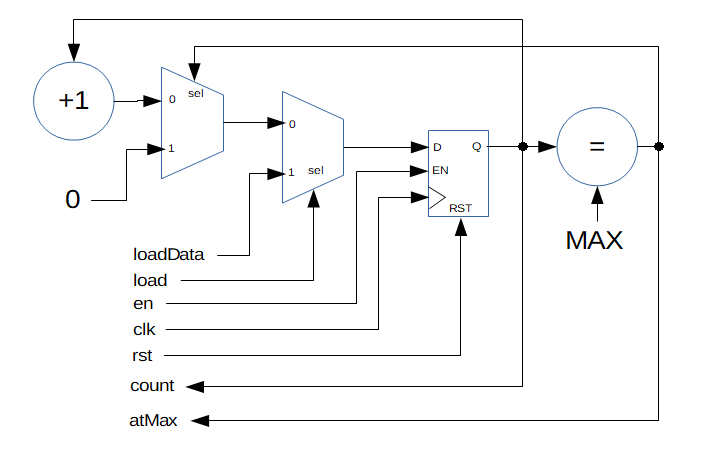
\includegraphics[width=15cm]{img/contador_bloque.png}
\captionof{figure}{Diagrama de Bloques de componente contador.}
\end{figure}

\subsection{sevenSegmentDisplay}

Este componente es un convertidor entre un cuatro bit BCD y los siete bits necesarios a mostrar la cifra en un display de siete segmentos.

\subsubsection{Señales y Parámetros}

\begin{tabular}{| l | l | r | p{8cm} |}
\hline
\textbf{Nombre} & \textbf{Tipo} & \textbf{Bits} & \textbf{Descripción} \\ \hline
\multicolumn{4}{|c|}{Entradas} \\ \hline
bcd & unsigned & 4 & Un numero entre 0 y 9. \\ \hline
\multicolumn{4}{|c|}{Salidas} \\ \hline
sevenSegmentOutput & unsigned & 7 & El patrón para mostrar el número BCD en el display de siete segmentos. \\ \hline
\end{tabular}

\subsubsection{Diagrama de Bloques}

\begin{figure}[!h]
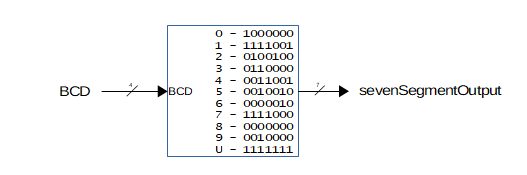
\includegraphics[width=15cm]{img/sevenSegmentDisplay_bloque.png}
\captionof{figure}{Diagrama de Bloques de componente sevenSegmentDisplay.}
\end{figure}

\subsection{tp1}

Este componente es el módulo de nivel más alto. Hay dos contadores que son generadores de enables, uno que genera un enable a 1Hz y el otro a 1KHz. Uso el de 1KHz para tener un modo rápido para mejor probar el diseño. Elijo cual a usar con un bóton en la placa DE2.

Después hay cuatro contadores más que cuentan entre cero y nueve. Cada uno corresponde a una cifra BCD. El enable del primero viene del generador de enable elegido por el bóton. Los otros están activos solo cuando el contador previo está activo y su valor es el máximo (9).

Cada uno de estos contadores conecta a la entrada de un sevenSegmentDisplay y la salida va al display de siete segmentos.

\subsubsection{Señales y Parámetros}

\begin{tabular}{| l | l | r | p{8cm} |}
\hline
\textbf{Nombre} & \textbf{Tipo} & \textbf{Bits} & \textbf{Descripción} \\ \hline
\multicolumn{4}{|c|}{Parámetros} \\ \hline
CLOCK\_DIVIDER & natural & & Esto es usado por el banco de pruebas para dejarme simular el diseño más rápidamente. \\ \hline
\multicolumn{4}{|c|}{Entradas} \\ \hline
KEY & std\_logic\_vector & 2 & Dos botones, uso uno para el reset, y el otro para activar módo rápido. Los dos están activa baja. \\ \hline
\multicolumn{4}{|c|}{Salidas} \\ \hline
HEX0 - HEX7 & std\_logic\_vector & 7 & Displays de siete segmentos. \\
\hline
\end{tabular}

\begin{minipage}{\textwidth}
\subsubsection{Diagrama de Bloques}

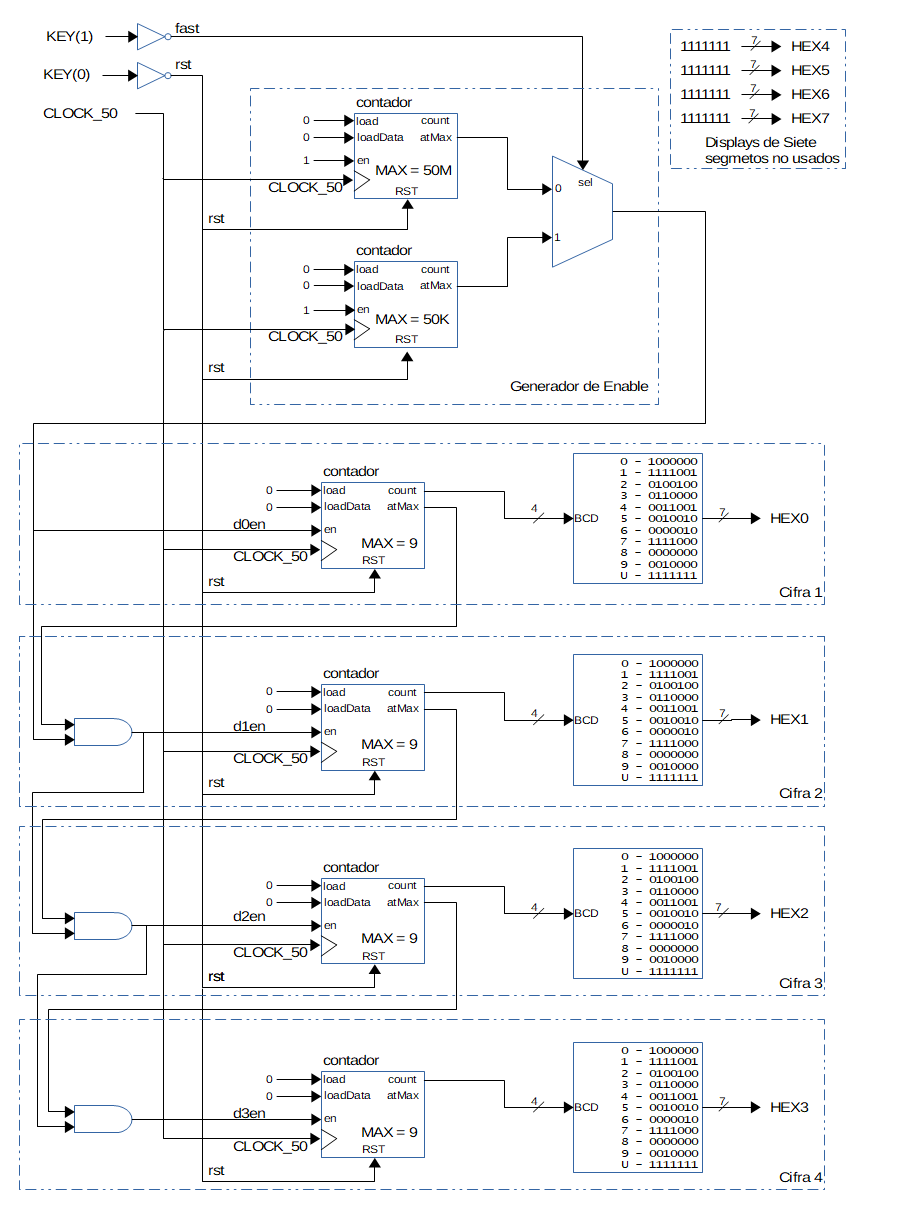
\includegraphics[width=14cm]{img/tp1_bloque.png}
\captionof{figure}{Diagrama de Bloques de componente tp1.}

\end{minipage}

\section{Simulación y Verificación}
Tengo bancos de pruebas para el contador y el tp1 que me permiten verificarlos. He usado asserts en PSL para especificar los requisitos y después estimulo las entradas para comprobar que todas las pruebas aprueban.

En el banco de prueba de tp1 en vez de solo comprobar las salidas del componente uso nombres jerárquicos para dejarme leer las salidas de los contadores que están señales internos de tp1.

Durante la simulación Questa Sim produce un mensaje para cada error y al final genera una tabla de resumen indicando cuantas fallas hubieron por cada assert.

También comprobé algunas partes interesantes de las olas generadas por Questa Sim.

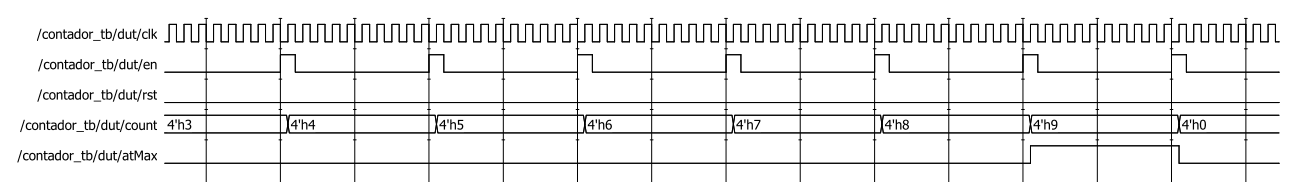
\includegraphics[width=15cm]{img/contador_waves.png}
\captionof{figure}{El contador solo cuenta cuando es activa.}

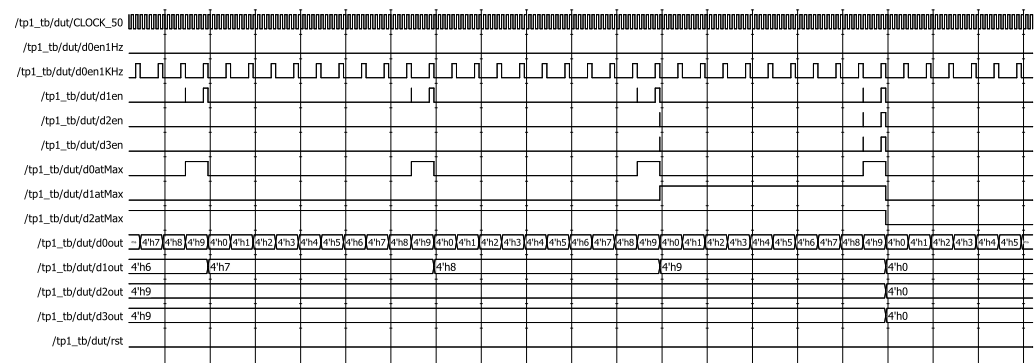
\includegraphics[width=15cm]{img/tp1_waves.png}
\captionof{figure}{Las cuatro cifras contando hasta 9999.}

\section{Síntesis}

He usado Quartus II para sintetizar el diseño.

\subsection{Resumen de síntesis}
\begin{tabular}{| l | r | r | r|}
\hline
\textbf{Ítem} & \textbf{Utilizado} & \textbf{Disponible} & \textbf{Porcentaje Utilizado} \\ \hline
Logic Elements & 126 & 33216 & \textless 1\% \\
Registers & 56 & 33216 & \textless 1\% \\
Global Clocks & 1 & 16 & 6\% \\ \hline
\end{tabular} \\

TimeQuest Timing Analyzer me informe que el frecuencia máxima de reloj a la que está operable el circuito es 145.54MHz.

\pagebreak
\section{Código}

Todo el código es disponible en mi github: \url{https://github.com/andrewparlane/fiuba6617/tree/master/TP1}.

\subsection{contador.vhd}
\begin{minted}{vhdl}
library ieee;
use ieee.std_logic_1164.all;
use ieee.numeric_std.all;

entity contador is
    generic (WIDTH: natural;
             MAX: natural);
    port (clk:      in  std_logic;
          en:       in  std_logic;
          rst:      in  std_logic;
          load:     in  std_logic;
          loadData: in  unsigned((WIDTH - 1) downto 0);
          count:    out unsigned((WIDTH - 1) downto 0);
          atMax:    out std_logic);
end entity contador;

architecture synth of contador is
    signal countAux: unsigned((WIDTH - 1) downto 0);
begin

    process (clk, rst)
    begin
        -- asíncrono reset
        if (rst = '1') then
            countAux <= (others => '0');
        elsif (rising_edge(clk)) then
            if (en = '1') then
                if (load = '1') then
                    countAux <= loadData;
                else
                    if (countAux = to_unsigned(MAX, WIDTH)) then
                        countAux <= (others => '0');
                    else
                        countAux <= countAux + to_unsigned(1, WIDTH);
                    end if;
                end if;
            end if;
        end if;
    end process;

    count <= countAux;
    atMax <= '1' when (countAux = MAX) else '0';

end architecture synth;
\end{minted}

\subsection{sevenSegmentDisplay.vhd}
\begin{minted}{vhdl}
library ieee;
use ieee.std_logic_1164.all;
use ieee.numeric_std.all;

entity sevenSegmentDisplay is
    port (bcd:                  in  unsigned(3 downto 0);
          sevenSegmentOutput:   out std_logic_vector(6 downto 0));
end entity sevenSegmentDisplay;

architecture synth of sevenSegmentDisplay is
    signal auxOut: std_logic_vector(6 downto 0);
begin

    -- los señales están activa baja.
    --
    --         0
    --      -------
    --      |     |
    --    5 |     | 1
    --      |  6  |
    --      -------
    --      |     |
    --    4 |     | 2
    --      |     |
    --      -------
    --         3

    with bcd select sevenSegmentOutput <=
            (not "0111111") when 4ux"0",
            (not "0000110") when 4ux"1",
            (not "1011011") when 4ux"2",
            (not "1001111") when 4ux"3",
            (not "1100110") when 4ux"4",
            (not "1101101") when 4ux"5",
            (not "1111101") when 4ux"6",
            (not "0000111") when 4ux"7",
            (not "1111111") when 4ux"8",
            (not "1101111") when 4ux"9",
            (not "0000000") when others;

end architecture synth;
\end{minted}

\subsection{tp1.vhd}
\begin{minted}{vhdl}
library ieee;
use ieee.std_logic_1164.all;
use ieee.numeric_std.all;

entity tp1 is
    generic (CLOCK_DIVIDER: natural := 1);
    port (CLOCK_50: in  std_logic;
          KEY:      in  std_logic_vector(1 downto 0);
          HEX0:     out std_logic_vector(6 downto 0);
          HEX1:     out std_logic_vector(6 downto 0);
          HEX2:     out std_logic_vector(6 downto 0);
          HEX3:     out std_logic_vector(6 downto 0);
          HEX4:     out std_logic_vector(6 downto 0);
          HEX5:     out std_logic_vector(6 downto 0);
          HEX6:     out std_logic_vector(6 downto 0);
          HEX7:     out std_logic_vector(6 downto 0));
end entity tp1;

architecture synth of tp1 is

    component contador is
        generic (WIDTH: natural;
                 MAX: natural);
        port (clk:      in  std_logic;
              en:       in  std_logic;
              rst:      in  std_logic;
              load:     in  std_logic;
              loadData: in  unsigned((WIDTH - 1) downto 0);
              count:    out unsigned((WIDTH - 1) downto 0);
              atMax:    out std_logic);
    end component contador;

    component sevenSegmentDisplay is
        port (bcd:                  in  unsigned(3 downto 0);
              sevenSegmentOutput:   out std_logic_vector(6 downto 0));
    end component sevenSegmentDisplay;

    -- Tenemos CLOCK_DIVIDER así que el banco de prueba
    -- no necesita simular 50.000.000 ticks para incrementar
    -- dígito 0 una vez.
    -- Usamos -1 aquí por que 0,1,2,3,4,5,0 es 6 ticks
    constant    ONE_HZ_EN_MAX:  natural := (50000000 / CLOCK_DIVIDER) - 1;
    constant    ONE_KHZ_EN_MAX: natural := (50000 / CLOCK_DIVIDER) - 1;

    signal d0en1Hz, d0en1KHz:           std_logic;
    signal d0en, d1en, d2en, d3en:      std_logic;
    signal d0atMax, d1atMax, d2atMax:   std_logic;
    signal d0out, d1out, d2out, d3out:  unsigned (3 downto 0);

    signal rst:                         std_logic;
    signal fast:                        std_logic;
begin

    -- HEX4,5,6,7 siempre están apagado
    HEX4 <= (others => '1');
    HEX5 <= (others => '1');
    HEX6 <= (others => '1');
    HEX7 <= (others => '1');

    -- KEY(0) es nRESET (activa baja).
    -- KEY(1) es para contar más rápido (activa baja).
    rst <= not KEY(0);
    fast <= not KEY(1);

    -- el primer dígito cuenta a 1Hz en modo normal,
    -- y 1KHz en modo rápido.
    d0en <= d0en1KHz when (fast = '1') else d0en1Hz;

    -- un dígito cuenta si el dígito anterior hace el transición 9 -> 0
    -- (en and atMax)
    d1en <= d0en and d0atMax;
    d2en <= d1en and d1atMax;
    d3en <= d2en and d2atMax;

    -- generar enable @ 1Hz desde 50MHz clk
    en1Hz_inst: contador
                generic map    (WIDTH => 26,
                                MAX => ONE_HZ_EN_MAX)
                port map       (clk => CLOCK_50,
                                en => '1',
                                rst => rst,
                                load => '0',
                                loadData => to_unsigned(0, 26),
                                -- count,
                                atMax => d0en1Hz);

    -- generar enable @ 1KHz desde 50MHz clk
    en1KHz_inst: contador
                 generic map   (WIDTH => 16,
                                MAX => ONE_KHZ_EN_MAX)
                 port map      (clk => CLOCK_50,
                                en => '1',
                                rst => rst,
                                load => '0',
                                loadData => to_unsigned(0, 16),
                                -- count,
                                atMax => d0en1KHz);

    -- dígito 0, 0-9
    d0Contador_inst:    contador
                        generic map    (WIDTH => 4,
                                        MAX => 9)
                        port map       (clk => CLOCK_50,
                                        en => d0en,
                                        rst => rst,
                                        load => '0',
                                        loadData => to_unsigned(0, 4),
                                        count => d0out,
                                        atMax => d0atMax);

    d0Display_inst:     sevenSegmentDisplay
                        port map       (bcd => d0out,
                                        sevenSegmentOutput => HEX0);

    -- dígito 1, 0-9
    d1Contador_inst:    contador
                        generic map    (WIDTH => 4,
                                        MAX => 9)
                        port map       (clk => CLOCK_50,
                                        en => d1en,
                                        rst => rst,
                                        load => '0',
                                        loadData => to_unsigned(0, 4),
                                        count => d1out,
                                        atMax => d1atMax);

    d1Display_inst:     sevenSegmentDisplay
                        port map       (bcd => d1out,
                                        sevenSegmentOutput => HEX1);

    -- dígito 2, 0-9
    d2Contador_inst:    contador
                        generic map    (WIDTH => 4,
                                        MAX => 9)
                        port map       (clk => CLOCK_50,
                                        en => d2en,
                                        rst => rst,
                                        load => '0',
                                        loadData => to_unsigned(0, 4),
                                        count => d2out,
                                        atMax => d2atMax);

    d2Display_inst:     sevenSegmentDisplay
                        port map       (bcd => d2out,
                                        sevenSegmentOutput => HEX2);

    -- dígito 3, 0-9
    d3Contador_inst:    contador
                        generic map    (WIDTH => 4,
                                        MAX => 9)
                        port map       (clk => CLOCK_50,
                                        en => d3en,
                                        rst => rst,
                                        load => '0',
                                        loadData => to_unsigned(0, 4),
                                        count => d3out);
                                        -- atMax,

    d3Display_inst:     sevenSegmentDisplay
                        port map       (bcd => d3out,
                                        sevenSegmentOutput => HEX3);

end architecture synth;
\end{minted}

\subsection{contador\_tb.vhd}
\begin{minted}{vhdl}
library ieee;
use ieee.std_logic_1164.all;
use ieee.numeric_std.all;

entity contador_tb is
end entity contador_tb;

architecture sim of contador_tb is

    component contador is
        generic (WIDTH: natural;
                 MAX: natural);
        port (clk:      in  std_logic;
              en:       in  std_logic;
              rst:      in  std_logic;
              load:     in  std_logic;
              loadData: in  unsigned((WIDTH - 1) downto 0);
              count:    out unsigned((WIDTH - 1) downto 0);
              atMax:    out std_logic);
    end component contador;

    constant WIDTH: natural := 4;
    constant MAX: natural := 9;

    -- dut señales
    signal clk:         std_logic := '0';
    signal rst:         std_logic := '1';
    signal en:          std_logic := '0';
    signal load:        std_logic := '0';
    signal loadData:    unsigned((WIDTH - 1) downto 0) := (others => '0');
    signal count:       unsigned((WIDTH - 1) downto 0);
    signal atMax:       std_logic;

begin

    -- clk period = 100ns
    clk <= not clk after 50 ns;

    dut: contador   generic map    (WIDTH => WIDTH,
                                    MAX => MAX)
                    port map       (clk => clk,
                                    rst => rst,
                                    en => en,
                                    load => load,
                                    loadData => loadData,
                                    count => count,
                                    atMax => atMax);

    process (count)
    begin
        report "count changed to " & integer'image(to_integer(count));
    end process;

    -- pruebas con PSL
    -- ---------------
    -- psl default clock is rising_edge(clk);
    --
    -- psl preubaRst:
    --      assert always rst -> next count = 0
    --      report "Failure: reset error";
    --
    -- psl preubaLoad:
    --      assert always (en and load) -> next count = loadData
    --      report "Failure: load error";
    --
    -- psl preubaMax:
    --      assert always (count = MAX) -> atMax
    --      report "Failure: atMax error - atMax not set when it should be";
    --
    -- psl preubaNMax:
    --      assert always (count /= MAX) -> not atMax
    --      report "Failure: atMax error - atMax set when it shouldn't be";
    --
    -- psl preubaCount:
    --      assert forall i in {0 to (MAX - 1)}:
    --          always ((count = i) and
    --                  (rst = '0') and
    --                  (load = '0') and
    --                  (en = '1'))
    --          -> next ((count = i + 1) or
    --                   (rst = '1') or
    --                   (load = '1'))
    --      report "Failure: counter error - didn't increment";
    --
    -- psl preubaCountOverflow:
    --      assert always ((count = MAX) and
    --                     (rst = '0') and
    --                     (load = '0') and
    --                     (en = '1'))
    --             -> next count = 0
    --      report "Failure: counter error - didn't overflow";
    --
    -- psl preubaEn:
    --      assert forall i in {0 to (MAX - 1)}:
    --          always ((count = i) and
    --                  (rst = '0') and
    --                  (en = '0'))
    --          -> next ((count = i) or
    --                   (rst = '1'))
    --      report "Failure: counter error - changed when en and rst were 0";

    process
    begin
        report "Comprobamos que o es 0 siempre cuándo estámos en reset";
        rst <= '1';
        en <= '0';
        wait for 500 ns;

        report "aun si en es 1";
        en <= '1';
        wait for 500 ns;

        report "contando cada tick";
        rst <= '0';
        wait for 3500 ns;

        report "se queda a loadData cuando load es alto";
        loadData <= to_unsigned(4, WIDTH);
        load <= '1';
        wait for 500 ns;

        report "y comenza desde load cuando load baja";
        load <= '0';
        wait for 1000 ns;

        report "nada pasa si load es alto hasta en es alto";
        load <= '1';
        en <= '0';
        wait for 500 ns;
        en <= '1';
        wait for 500 ns;
        load <= '0';
        wait for 500 ns;

        report "en sólo alto una vez cada 10 ticks";
        rst <= '1';
        wait for 100 ns;
        rst <= '0';
        for i in 0 to 40 loop
            en <= '0';
            wait for 900 ns;
            en <= '1';
            wait for 100 ns;
        end loop;

        std.env.stop;
    end process;

end architecture sim;
\end{minted}

\subsection{tp1\_tb.vhd}
\begin{minted}{vhdl}
library ieee;
use ieee.std_logic_1164.all;
use ieee.numeric_std.all;

entity tp1_tb is
end entity tp1_tb;

architecture sim of tp1_tb is

    component tp1 is
        generic (CLOCK_DIVIDER:  natural);
        port (CLOCK_50: in  std_logic;
              KEY:      in  std_logic_vector(1 downto 0);
              HEX0:     out std_logic_vector(6 downto 0);
              HEX1:     out std_logic_vector(6 downto 0);
              HEX2:     out std_logic_vector(6 downto 0);
              HEX3:     out std_logic_vector(6 downto 0));
    end component tp1;

    signal clk:         std_logic   := '0';
    signal nRst:        std_logic   := '0';
    signal nFast:       std_logic   := '1';
    signal key:         std_logic_vector(1 downto 0) := "00";

    -- usamos esto por los outputs de los contadores
    type countsArray is array (3 downto 0) of unsigned(3 downto 0);
    signal counts: countsArray;

begin

    -- clk = 50MHz => periodo = 20ns
    clk <= not clk after 10 ns;

    -- key
    key <= nFast & nRst;

    dut:    tp1 generic map    (CLOCK_DIVIDER => 10000)   -- incrementar el primer dígito cada 5000 ticks
                port map       (CLOCK_50 => clk,
                                KEY => key);

    -- leer las salidas de las contadores en tp1.
    counts(0) <= <<signal dut.d0out: unsigned(3 downto 0)>>;
    counts(1) <= <<signal dut.d1out: unsigned(3 downto 0)>>;
    counts(2) <= <<signal dut.d2out: unsigned(3 downto 0)>>;
    counts(3) <= <<signal dut.d3out: unsigned(3 downto 0)>>;

    -- pruebas con PSL
    -- ---------------
    -- psl default clock is rising_edge(clk);
    --
    enRstGenerate: for c in 0 to 3 generate
        type ticksEntreCambioArray is array (0 to 3) of natural;
        constant fastTicksEntreCambio: ticksEntreCambioArray
                                    := (5, 50, 500, 5000);
        constant normalTicksEntreCambio: ticksEntreCambioArray
                                    := (5000, 50000, 500000, 5000000);
    begin
        -- ----------------------------------------------------------
        -- si estamos en rst todo los counts debería estar 0
        -- ----------------------------------------------------------
        -- psl enRst:
        --      assert always (nRst = '0') ->
        --                    (counts(c) = 0)
        --      report "Error: counts(c) != 0 cuando en reset";
        -- ----------------------------------------------------------
        --
        -- ----------------------------------------------------------
        -- en modo rápido cada fastTicksEntreCambio(c) counts(c)
        -- deberia incrementar
        -- ----------------------------------------------------------
        -- psl fastCount:
        --      assert forall i in {0 to 8}:
        --          always ((counts(c) = i) and
        --                  (nFast = '0') and
        --                  (nRst = '1'))
        --          -> next[fastTicksEntreCambio(c)]
        --             (counts(c) = i + 1)
        --             abort ((nRst = '0') or
        --                    (nFast = '1'))
        --      report "Error: counts(c) modo rápido no cuenta correcto";
        -- ----------------------------------------------------------
        --
        -- ----------------------------------------------------------
        -- en modo rápido si counts(c) es 9, en
        -- fastTicksEntreCambio(c) ticks count(c)
        -- debería estar 0
        -- ----------------------------------------------------------
        -- psl fastOverflow:
        --      assert always ((counts(c) = 9) and
        --                     (nFast = '0') and
        --                     (nRst = '1'))
        --             -> next[fastTicksEntreCambio(c)]
        --                (counts(c) = 0)
        --                abort ((nRst = '0') or
        --                       (nFast = '1'))
        --      report "Error: counts(c) modo rápido no hizo overflow";
        -- ----------------------------------------------------------
        --
        -- ----------------------------------------------------------
        -- en modo normal cada normalTicksEntreCambio(c) counts(c)
        -- deberia incrementar
        -- ----------------------------------------------------------
        -- psl normalCount:
        --      assert forall i in {0 to 8}:
        --          always ((counts(c) = i) and
        --                  (nFast = '1') and
        --                  (nRst = '1'))
        --          -> next[normalTicksEntreCambio(c)]
        --             (counts(c) = i + 1)
        --             abort ((nRst = '0') or
        --                    (nFast = '0'))
        --      report "Error: counts(c) modo normal no cuenta correcto";
        -- ----------------------------------------------------------
        --
        -- ----------------------------------------------------------
        -- en modo rápido si counts(c) es 9, en
        -- fastTicksEntreCambio(c) ticks count(c)
        -- debería estar 0
        -- ----------------------------------------------------------
        -- psl normalOverflow:
        --      assert always ((counts(c) = 9) and
        --                     (nFast = '1') and
        --                     (nRst = '1'))
        --             -> next[normalTicksEntreCambio(c)]
        --                (counts(c) = 0)
        --                abort ((nRst = '0') or
        --                       (nFast = '0'))
        --      report "Error: counts(c) modo normal no hizo overflow";
        -- ----------------------------------------------------------
    end generate;

    process
    begin
        -- recuerdes que los keys son activa baja
        -- reset
        nRst <= '0';
        wait for 100 ns;

        -- no es suficiente a overflow 9999 -> 0000
        -- pero es bastante para mostrar que funciona bien
        -- en modo normal. Y podríamos comprobar los dígitos
        -- altos y el overflow en modo rapido
        -- 10 * 5,000 ticks * 20ns = 1ms
        nRst <= '1';
        nFast <= '1';
        wait for 1100 us;

        -- hacemos una prueba más completo en modo rápido
        -- 10,000 * 5 tics * 20ns = 1ms
        nFast <= '0';
        wait for 1100 us;

        std.env.stop;
    end process;

end architecture sim;
\end{minted}
\end{document}
